
\chapter{HPS Signal and Backgrounds}

The Heavy Photon Search is a fixed target experiment that will search for heavy
photons in the mass range of 20 MeV/c$^{2}$ to 500 MeV/c$^{2}$ and couplings
of $\epsilon \sim 10^{-5} - 10^{-1}$.  Since heavy photons couple to electric
charge, they can be produced by a process analogous to bremsstrahlung 
radiation.  The heavy photon subsequently decays to narrow $e^+e^-$ resonances, 
which can be observed above the dominant quantum electrodynamic (QED) trident
background.  For suitably small couplings, heavy photons travel detectable 
distances before decaying providing an additional search channel.  In the 
chapter that follows, both the heavy photon production mechanism and backgrounds
will be discussed.

\section{Production of Heavy Photons}

Sensitivity to the theoretically favored regions of the heavy photon 
mass-coupling phase space can be best achieved using high luminosity fixed
target experiments \cite{Bjorken:2009mm}.  In such experiments, an electron
of energy $E_{0}$ incident on a high $Z$ target will radiate heavy photons 
through a process analogous to ordinary photon bremsstrahlung. 
%
% Do I need to explain what bremsstrahlung is or should I assume it's common
% knowledge?
%
However, as discussed below, the weak coupling
of the $A'$ to electrons along with its relatively large mass will lead to 
rates and kinematics which are very different from ordinary photon 
bremsstrahlung.

Consider the process shown on Fig. \ref{fig:ap_production} where an $A'$ with
momentum $k = (E_{A'}, \vec{k})$ is radiated by an electron of momentum 
$p = (E_0, \vec{p})$ incident on a target of mass $M_i$ and momentum 
$P_i = (M_i, 0)$. The energy-angle distribution of heavy photons produced in 
such a reaction can be estimated using the Weizacker-Williams approximation (WWA)
%%%%%%%%%%%%%%
%   Figure   %
%%%%%%%%%%%%%%
\begin{figure}[t]
    \centering
    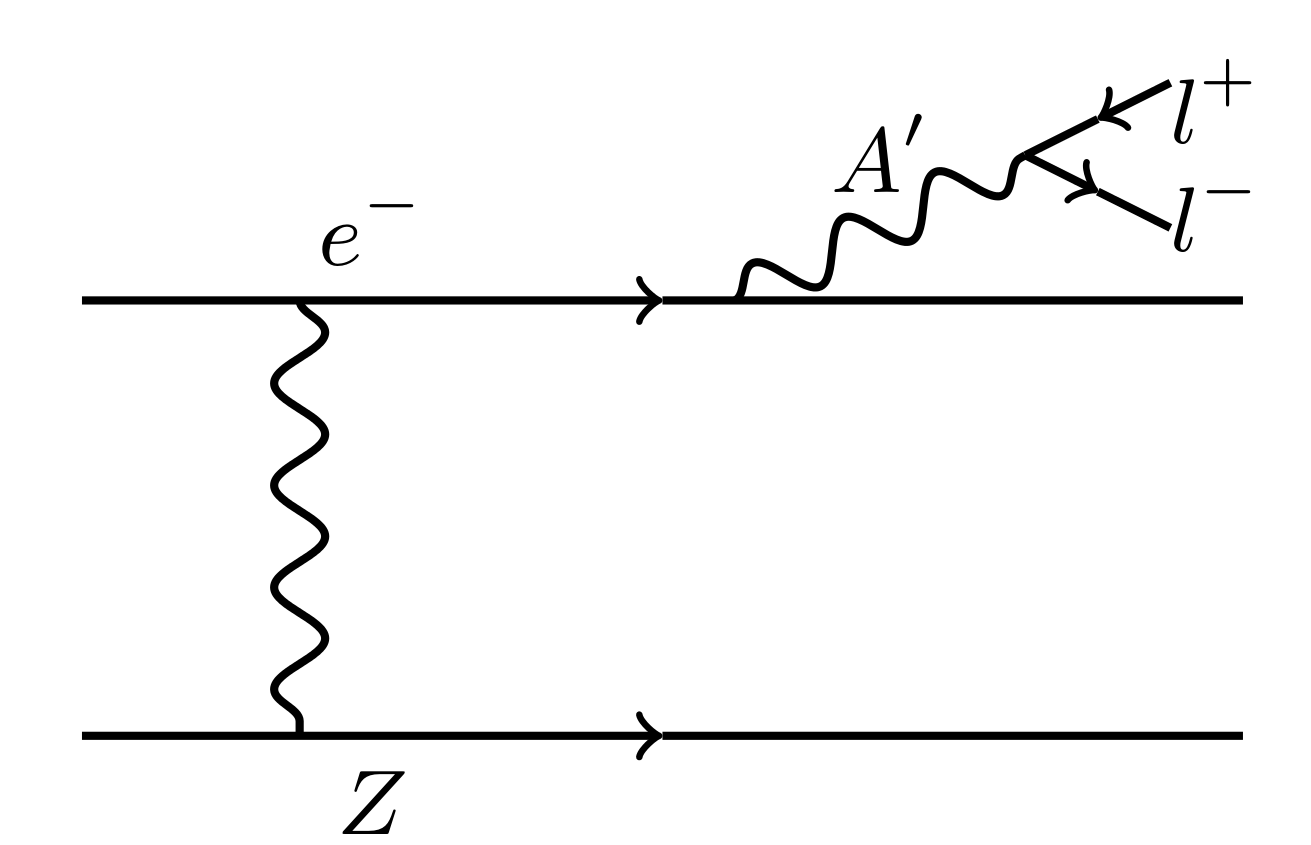
\includegraphics[width=0.5\textwidth]{images/aprime_brem.png}
    \caption{A heavy photon can be produced through a process analogous to 
             ordinary photon bremsstrahlung.}
    \label{fig:ap_production}
\end{figure}  
%%%%%%%%%%%%%%
%%%%%%%%%%%%%%
\cite{Bjorken:2009mm, Tsai:1986tx}.  The WWA models the process as the 
scattering of photons sourced by the target nuclei by the incident electron
in the rest frame of the electron.  Therefore, the energy-angle distribution
can be obtained from the Compton-like process as
\begin{equation}
    \begin{split}
        \left[ \frac{d\sigma(e(p) + Z(P_i) \rightarrow e(p') + A'(k) + Z(P_f))}{dx d\cos\theta_{A'}} \right]_{\text{W.W.}} = \\
        \left( \frac{\alpha \chi}{\pi} \right) \left(\frac{E_0 x \sqrt{ 1 - m_{A'}^2/E_0^2}}{(1 - x)} \right) 
        \frac{d\sigma(e(p)\gamma(q) \rightarrow e(p') A'(k))}{d(p \cdot k)} |_{t = t_{\text{min}}} = \\
    \frac{8 \alpha^{3} \epsilon^{2} E_{0}^2 x \sqrt{1-m_{A'}^{2}/E_{0}^{2}}}{U^{2}} \chi
    \left [ \left (1 - x + \frac{x^{2}}{2} \right )  - \frac{(1-x)^{2} m_{A'}^{2}}{U^{2}}
    \left(m_{A'}^{2} - \frac{Ux}{1-x} \right) \right]
    \end{split}
    \label{eqn:ap_diff_cross}
\end{equation}
where $P_f$ and $p' = (E', \vec{p'})$ are the final momentum of the electron
and target respectively, $t = -q^2 = -(P_{i} - P_{f})^2$ is the momentum transfer, 
$\alpha \sim 1/137$ is the fine structure constant, $\theta_{A}$ is the
opening angle of the $A'$ relative to the incident electron in the lab frame, 
$x = E_{A'}/E_{0}$ is the fraction of the incident electron energy carried by
the $A'$, $m_A'$ is the mass of the heavy photon. The function 
\begin{equation}
    U(x, \theta_{A'}) = E_{0}^{2}x\theta_{A'}^{2} 
    + m_{A'}^{2}\frac{1-x}{x} + m_{e}^2 x
\end{equation}
is related to the virtuality of the intermediate electron.  The WW effective
photon flux, $\chi$, is related to the electric form factor as
\begin{equation}
    \chi = \int_{t_{\text{min}}}^{t_{\text{max}}} \left(G_{2,\text{el}}(t) + G_{2,\text{in}}(t) \right) \frac{t - t_{\text{min}}}{t^2} dt
\end{equation}
where $G_{2,\text{el}}$ is the elastic form factor, $G_{2,\text{in}}$ is the inelastic form
factor, $t_{min} = (m^2_{A'}/2E_{0})^2$ and $t_{max} = m_{A'}^2$.  Both the 
elastic and inelastic form factors parameterize effects due to electron screening
and the size of the nucleus.  Their exact forms are given in the appendix of 
\cite{Bjorken:2009mm}.  For the conditions during the engineering run, a reduced
WW effective photon flux in the range $\chi^2/Z^2 \sim 5 - 10$ is expected.
%where the elastic component is given by
%\begin{equation}
%    G_{2, el}(t) = \left(\frac{a^2t}{1+a^2t}\right)^2\left(\frac{1}{1+t/d}\right)^2Z^2
%\end{equation}
%and the inelastic term by
%\begin{equation}
%    G_{2,in}(t) = \left(\frac{a'^2t}{1+a'^2t}\right)^2\left(\frac{1+\frac{t}{4m_{p}}(\mu_p^2 - 1)}
%                    {(1+\frac{t}{0.71 GeV^2})^4}\right)^2Z
%\end{equation}

Assuming $m_{e} << m_{A'}$, 
and integrating \ref{eqn:ap_diff_cross} over all angles yields
\begin{equation}
    \label{eqn:ap_diff_cross_i}
    \frac{d\sigma}{dx} = \frac{8\alpha^{3}\epsilon^{2} \sqrt{1-m_{A'}^{2}/E_{0}^{2}}}
    {m_{A'}^{2}\frac{1-x}{x} + m_{e}^{2}x}\chi
    \left( 1 - x + \frac{x^{2}}{3}\right).
\end{equation}
Although \ref{eqn:ap_diff_cross_i} reduces to the cross-section of photon 
bremsstrahlung in the limit that $m_{A'} \rightarrow 0$, their production rate
and kinematics differ in several ways: 
\begin{itemize}
    \item As can been seen from equation \ref{eqn:ap_diff_cross_i}, the rate of 
          production of heavy photons is $\propto \frac{\alpha^3 \epsilon^2}{m_{A'}^2}$.
          This implies that it is suppressed by a factor of 
          $\frac{\epsilon^{2}m_{e}^{2}}{m_{A'}^{2}}$ relative to ordinary photon 
          bremsstrahlung.
    \item The WW effective photon flux has a sharp turn off as the mass of the 
          $A'$ increases or the energy of the incident beam decreases further
          suppressing the production cross-section in these cases.  For the 
          HPS engineering run, the turn off occurs at around 400 MeV.
    \item The $A'$ production rate is maximized when $x \approx 1$ since 
          $U(x, 0)$  is minimized.  As a result, when an $A'$ is produced, 
          it will carry most of the beam energy.
      \item The emission angle of the heavy photon has a cutoff given by 
          \begin{equation}
              \theta_{A', \text{max}} \sim \text{max}\left(\frac{\sqrt{m_{A'}m_e}}{E_0}, 
              \frac{m_{A'}^{3/2}}{E_{0}^{3/2}}\right)
          \end{equation}
          which is much smaller than the opening angle of the decay products of
          the $A'$, $\sim m_{A'}/E_{0}$. 
\end{itemize}


Equation \ref{eqn:ap_diff_cross_i} can be used to derive an expression for the
number of heavy photons produced when $N_{e^-}$ electrons scatter in a
thin-target of radiation length, $T \ll 1$ as  
\begin{equation}
        N_{A'} \sim N_{e^-}\frac{N_0X_0}{A}T\frac{Z^2\alpha^3\epsilon^2}{m_{A'}^2}\frac{\chi}{Z^2}
\end{equation}
where $N_0$ is Avogadro's number, $X_0$ is the radiation length of the target
and $A$ is the atomic mass \cite{Bjorken:2009mm}.  Figure \ref{fig:ap_rate} shows
an estimated of the expected number of $A'$ events as a function of $A'$ mass 
and $\epsilon$ given the unblinded portion of the HPS engineering run data.
\begin{figure}[t]
    \centering
    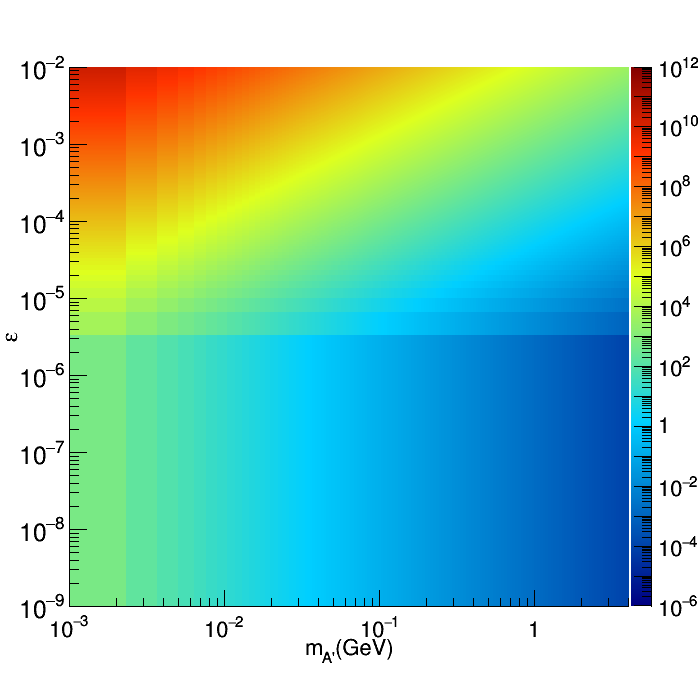
\includegraphics[width=0.8\textwidth]{images/20160517_rate.png}
    \caption{The expected number of $A'$ events given the unblinded portion of
             the engineering run data.}
    \label{fig:ap_rate}
\end{figure}  

\section{Trident Backgrounds}

The primary background expected to dominate the final event sample of the HPS 
experiment is the QED Bethe-Heitler and radiative trident processes.  Diagrams
of these processes are shown in Fig. \ref{fig:tridents}. The heavy photon 
signal is expected to appear as a resonance above the trident invariant mass
distribution so an understanding of these backgrounds is highly desirable. 
\begin{figure}[t]
    \begin{subfigure}{.5\textwidth}
        \centering
        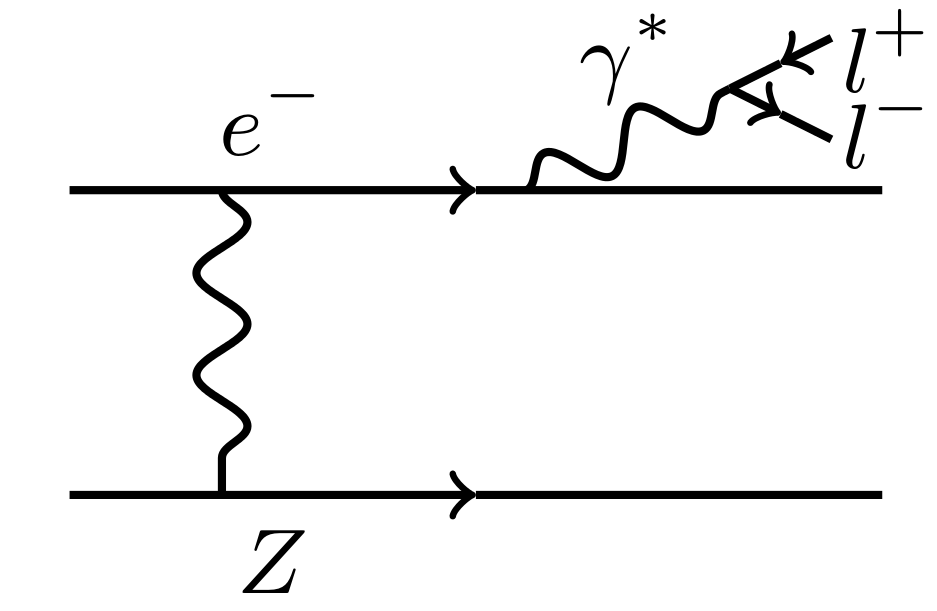
\includegraphics[width=0.8\textwidth]{images/radiative.png}
    \end{subfigure}
    \begin{subfigure}{.5\textwidth}
        \centering
        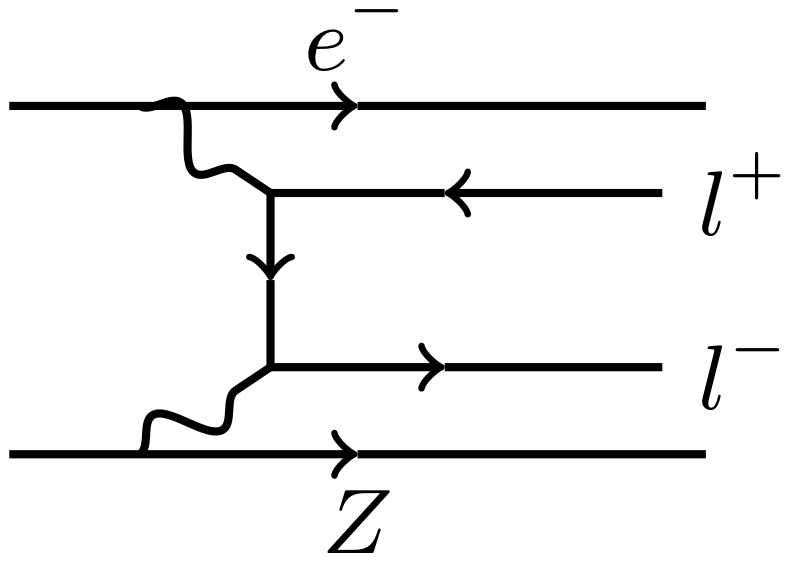
\includegraphics[width=0.8\textwidth]{images/bethe-heitler.png}
    \end{subfigure}
    \caption{Diagrams of the radiative and Bethe-Heitler trident reactions.}
    \label{fig:tridents}
\end{figure}  

The kinematics of radiatives are indistinguishable from $A'$ signal events 
within an invariant mass window, $\delta m$, near $m_{A'}$. Specifically, 
the $A'$ production cross-section is related to the production cross-section of 
radiatives as 
\begin{equation}
    \frac{d\sigma(e^-Z\rightarrow e-Z(A'\rightarrow l^+l^-))}
    {d\sigma(e^-Z\rightarrow e-Z(\gamma^*\rightarrow l^+l^-))}
    = \frac{3\pi\epsilon^{2}}{2 N_{eff} \alpha} \frac{m_{A'}}{\delta m}
\end{equation}
where $N_{\text{eff}}$ is the number of decay channels available.
Therefore, radiatives can be used to analyze both the rate of the $A'$ signal 
production and the sensitivity of an experiment to $A'$ signals.

Although the rate of the Bethe-Heitler process dominates among the two 
processes, its different kinematics can be used to reduce them in the final 
event sample.  Specifically, the $A'$ decay products are highly boosted while 
the recoiling electron is soft and scatters at large angles.  In contrast, 
at higher energies, the Bethe-Heitler process is not enhance.  Furthermore,
only one of the leptons in the pair will be highly boosted, while the other
will be much softer.  As a result, the recoiling electron will be produced much more forward.
These kinematic differences are illustrated in Figure \ref{fig:ap_v_bethe} which
shows the energy of the positron versus the electron energy for both $A'$ (red)
and Bethe-Heitler (black) events.  As can be seen from the figure, the signal
distribution is concentrated in the region where the sum of the energy of the
electron and positron is approximately equal to the beam energy.
\begin{figure}[b]
    \centering
    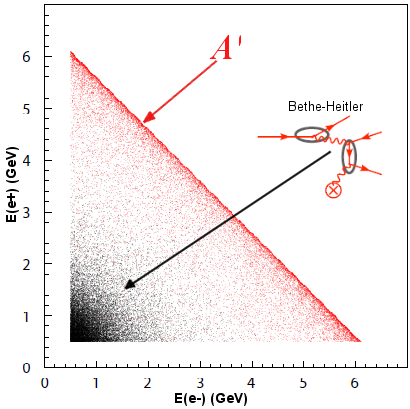
\includegraphics[width=0.5\textwidth]{images/bh_energy_cut.png}
    \caption{The distribution of the energy of the positron versus the electron
    for Bethe-Heitler (black) and $A'$ (red) event.}
    \label{fig:ap_v_bethe}
\end{figure}


